\documentclass[aspectratio=169]{beamer} % 16:9 aspect ratio for modern screens

% Theme settings
\usetheme[progressbar=foot]{metropolis} % Minimalist theme
\metroset{progressbar=frametitle} % Progress bar soll nur folien mit titel berücksichtigen?
\setbeamercolor{background canvas}{bg=white} % White background color

\makeatletter
    \setlength{\metropolis@progressinheadfoot@linewidth}{1.5pt}
\makeatother


\usefonttheme{professionalfonts} % Font theme

% Packages
\usepackage[T1]{fontenc}   % Font encoding
\usepackage[ngerman]{babel} % German language
\usepackage[sfdefault]{FiraSans} % For FiraSans font
\usepackage[backend=biber, style=authoryear-comp
, sorting=nyt]{biblatex} % For bibliography
\usepackage{csquotes} % Recommended for biblatex with babel/polyglossia
\usepackage{textgreek} % Greek letters in text mode (aus references von Citavi)
\usepackage{tikz}          % For drawing graphics

\usepackage{graphicx}       % For including images
\usepackage{amsmath, amssymb} % For math symbols

\usepackage[labelformat=empty]{caption}


% Bibliography settings
\addbibresource{references.bib} % Path to the bibliography file

% custom Citation commands
\DeclareCiteCommand{\citeauthortitle}
  {\usebibmacro{prenote}}
  {\usebibmacro{citeindex}%
   \printnames{labelname}%
   \setunit{\space\textendash\space}
   \printfield{title}}
  {\multicitedelim}
  {\usebibmacro{postnote}}

  \DeclareCiteCommand{\citeauthortitleurl}
  {\usebibmacro{prenote}}
  {\usebibmacro{citeindex}%
   \printnames{labelname}%
   \setunit{\space\textendash\space}
   \printfield{title}%
   \setunit{\addsemicolon\space}
   \printfield{url}}
  {\multicitedelim}
  {\usebibmacro{postnote}}

\DeclareCiteCommand{\parenciteauthortitle}
  {\usebibmacro{prenote}}
  {\bibopenparen\usebibmacro{citeindex}%
   \printnames{labelname}%
   \setunit{\space\textendash\space}% <- Hier wird das Trennzeichen ":" hinzugefügt
   \printfield{title}\bibcloseparen}
  {\multicitedelim}
  {\usebibmacro{postnote}}

\makeatletter
\renewcommand\footnotesize{\tiny}
\makeatother

\newcommand{\figcite}[1]{\\[-3mm]{\tiny Quelle: \cite{#1}}}
\newcommand{\figciteweb}[1]{\\[-3mm]{\tiny aus: \citeauthortitle{#1}}}
\newcommand{\figciteweburl}[1]{\\[-3mm]{\tiny aus: \citeauthortitleurl{#1}}}
  
% Title page settings
\title{Hadronen im Quarkmodell}
\subtitle{Wissenschaftliches Präsentieren}
\author{Florian Adamczyk}
\date{\today}

\begin{document}

    % Black slide
    \begin{frame}[plain, noframenumbering]
        \begin{tikzpicture}[remember picture, overlay]
            \fill[black] (current page.south west) rectangle (current page.north east);
        \end{tikzpicture}
    \end{frame}

    % Appetizer Slide
    \begin{frame}[noframenumbering, plain]{Eine Reise in den Zoo der Teilchen}
        \centering
        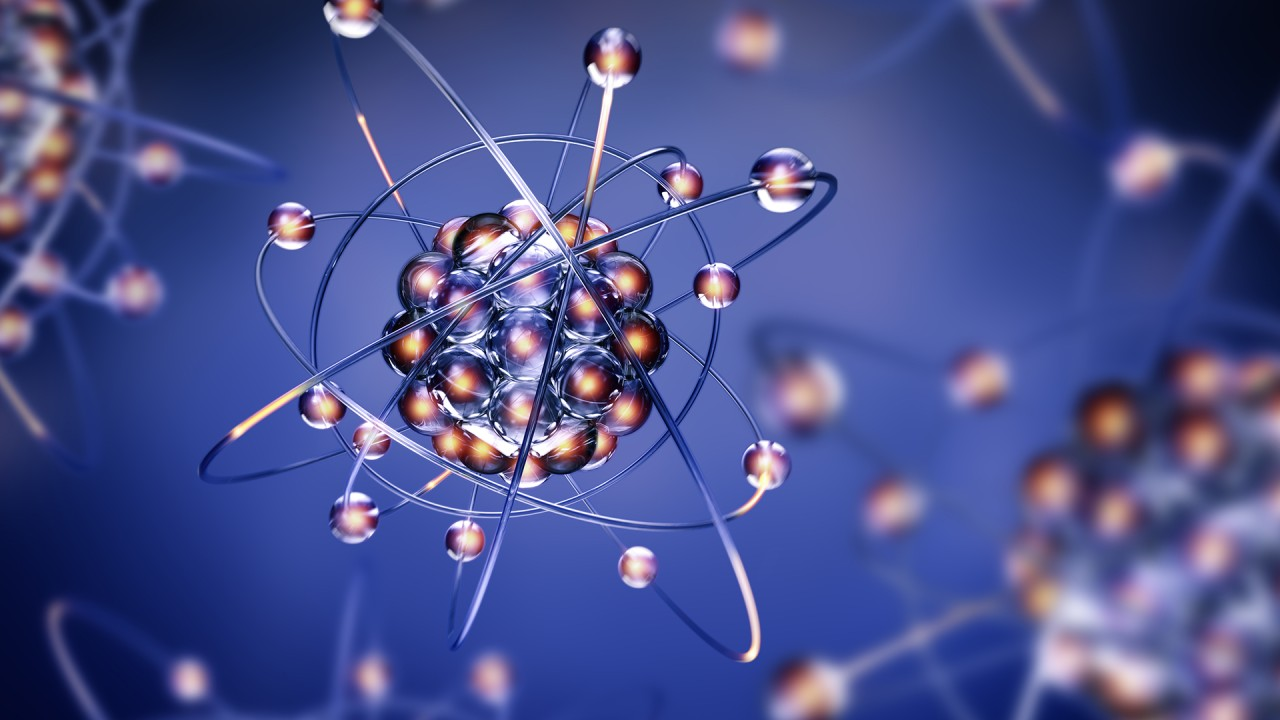
\includegraphics[width=\textwidth, height=0.9\textheight, keepaspectratio]{atom.jpg}
        \figciteweburl{Bonn.19.08.2021}
        % \vspace{0.5cm}
        % \begin{quote}
%{Stellen Sie sich vor, das Universum ist ein riesiger Zoo, bevölkert mit einer unglaublichen Vielfalt an exotischen Lebewesen – den Teilchen. Einige sind uns vertraut, wie Elektronen oder Protonen, aber es gibt auch faszinierende, kurzlebige Kreaturen. Eine Gruppe davon sind die Hadronen, die ich euch heute Vorstellen möchte.}
        % \end{quote}
    \end{frame}

    % Title Slide
    \begin{frame}[noframenumbering, plain]
        \vspace*{-0.6cm}
        \titlepage
        \vspace*{-1.6cm}
    \end{frame}
    
    % Table of Contents
    \begin{frame}{Gliederung}
      \setcounter{page}{1}
        \tableofcontents
    \end{frame}
    
    \section{Einführung}
    \begin{frame}{Das Standardmodell der Elementarteilchen}
      \begin{figure}
        \centering
        \begin{minipage}{0.5\textwidth}
          \centering
          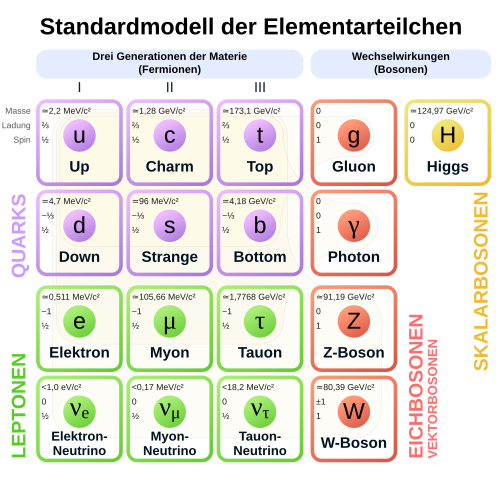
\includegraphics[width=\textwidth, keepaspectratio, height=0.85\textheight]{502px-Standard_Model_of_Elementary_Particles-de.svg.png}\tiny
          \figciteweb{Wikipedia.Standardmodell}, \citeurl{Wikipedia.Standardmodell} \end{minipage}
        \hfill
        \begin{minipage}{0.48\textwidth}
          \begin{itemize}
            \item Beschreibt Elementarteilchen \& Wechselwirkungen
            \item Fermionen (Quarks, Leptonen) \& Bosonen (Vektorbosonen, Higgs-Boson)
            \item Starke, schwache \& elektromagnetische Wechselwirkung
          \end{itemize}
          \end{minipage}
      \end{figure}
    \end{frame}

    \section{Hadronen}
    \begin{frame}{Hadronen: Aufbau und Klassifizierung}
      \begin{itemize}
        \item Baryonen (drei Quarks: Proton, Neutron, \dots)
        \item Mesonen ($q\bar{q}$, z.B. Pion, Kaon, \dots)
        \item Zusammengesetzt aus Quarks (durch starke WW gebunden)
        \item Unterliegen Quantenzahlen (Isospin, Strangeness, \dots)
      \end{itemize}
      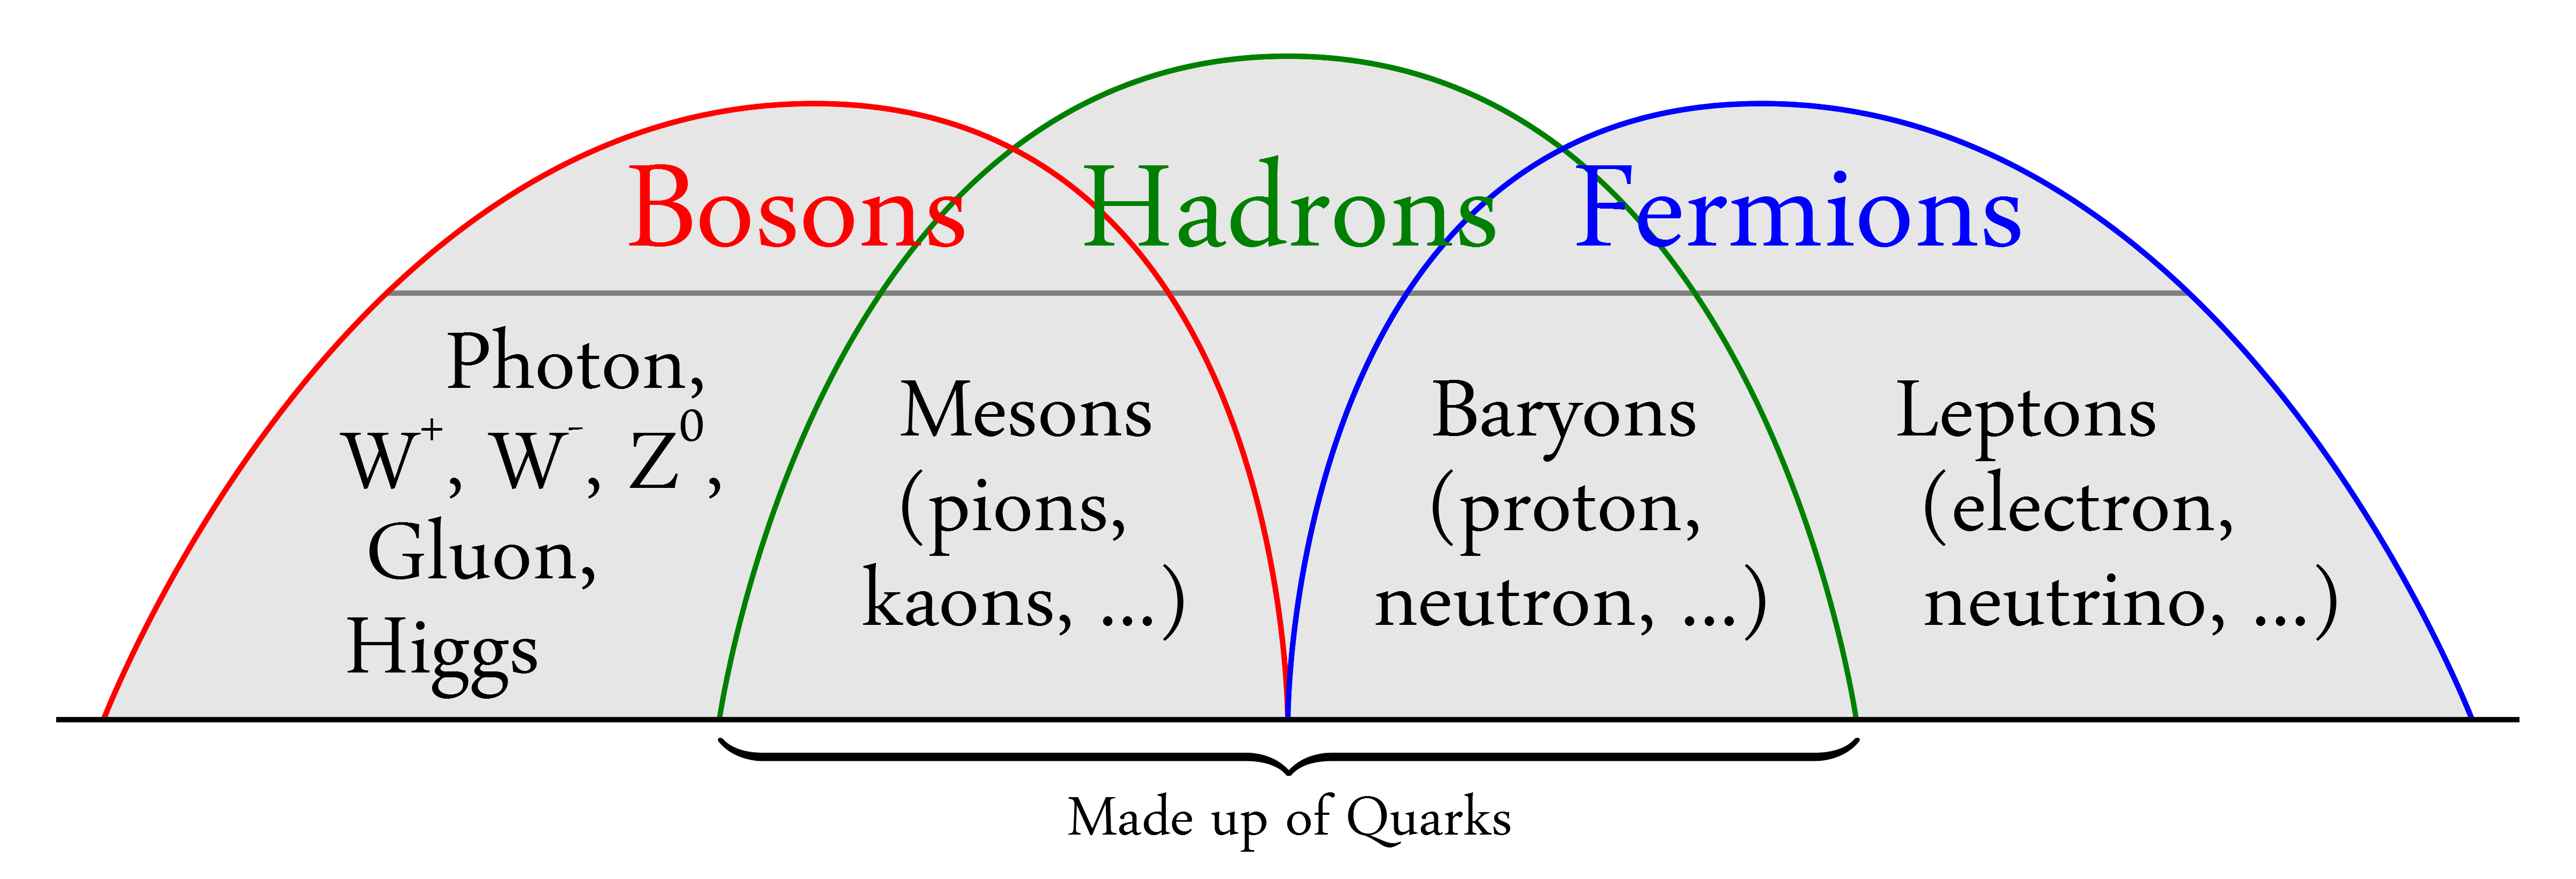
\includegraphics[width=\textwidth, height=0.4\textheight, keepaspectratio]{Bosons-Hadrons-Fermions-RGB-png2.png}
      \figciteweburl{Wikipedia.Hadron}
    \end{frame}

    \subsection{Das SU$_3$ Dekuplett}
    \begin{frame}{Das SU\(_3\) Dekuplett}
        \begin{minipage}{0.6\textwidth}
          \begin{figure}
            \centering
          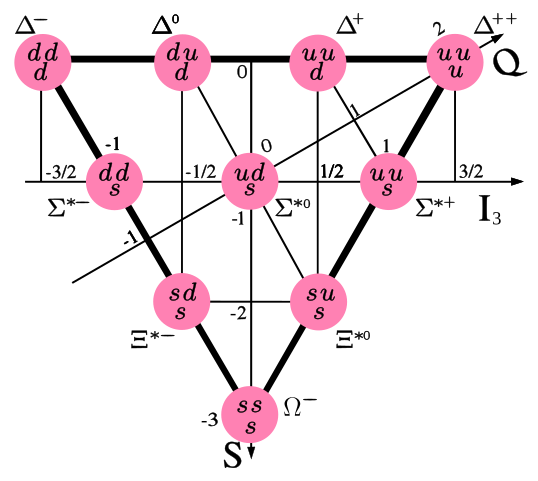
\includegraphics[width=\linewidth, keepaspectratio, height=0.8\textheight]{538px-Baryon-decuplet-small.svg.png}
          \tiny \\\citeauthortitle{Wikipedia.DeltaBaryon}, \citeurl{Wikipedia.DeltaBaryon}
      \end{figure}
        \end{minipage}
        \hfill
        \begin{minipage}{0.38\textwidth}
          \begin{itemize}
            \item I$_3$: Isospin
            \item S: Strangeness
            \item Q: Hyperladung % Grundzustand, parallele Spins und selben Falvour: Pauli Prinzip!!
          \end{itemize}
          \vspace*{2cm}
          \normalsize{\textbf{{$\rightarrow$ Einführung der \emph{Farbladung}}}}\vspace*{1cm}
        \end{minipage}
    \end{frame}
    
    \begin{frame}{Erweiterung des SU\(_3\) Dekupletts}
      \begin{minipage}{0.6\textwidth}
      \begin{figure}
        \centering
        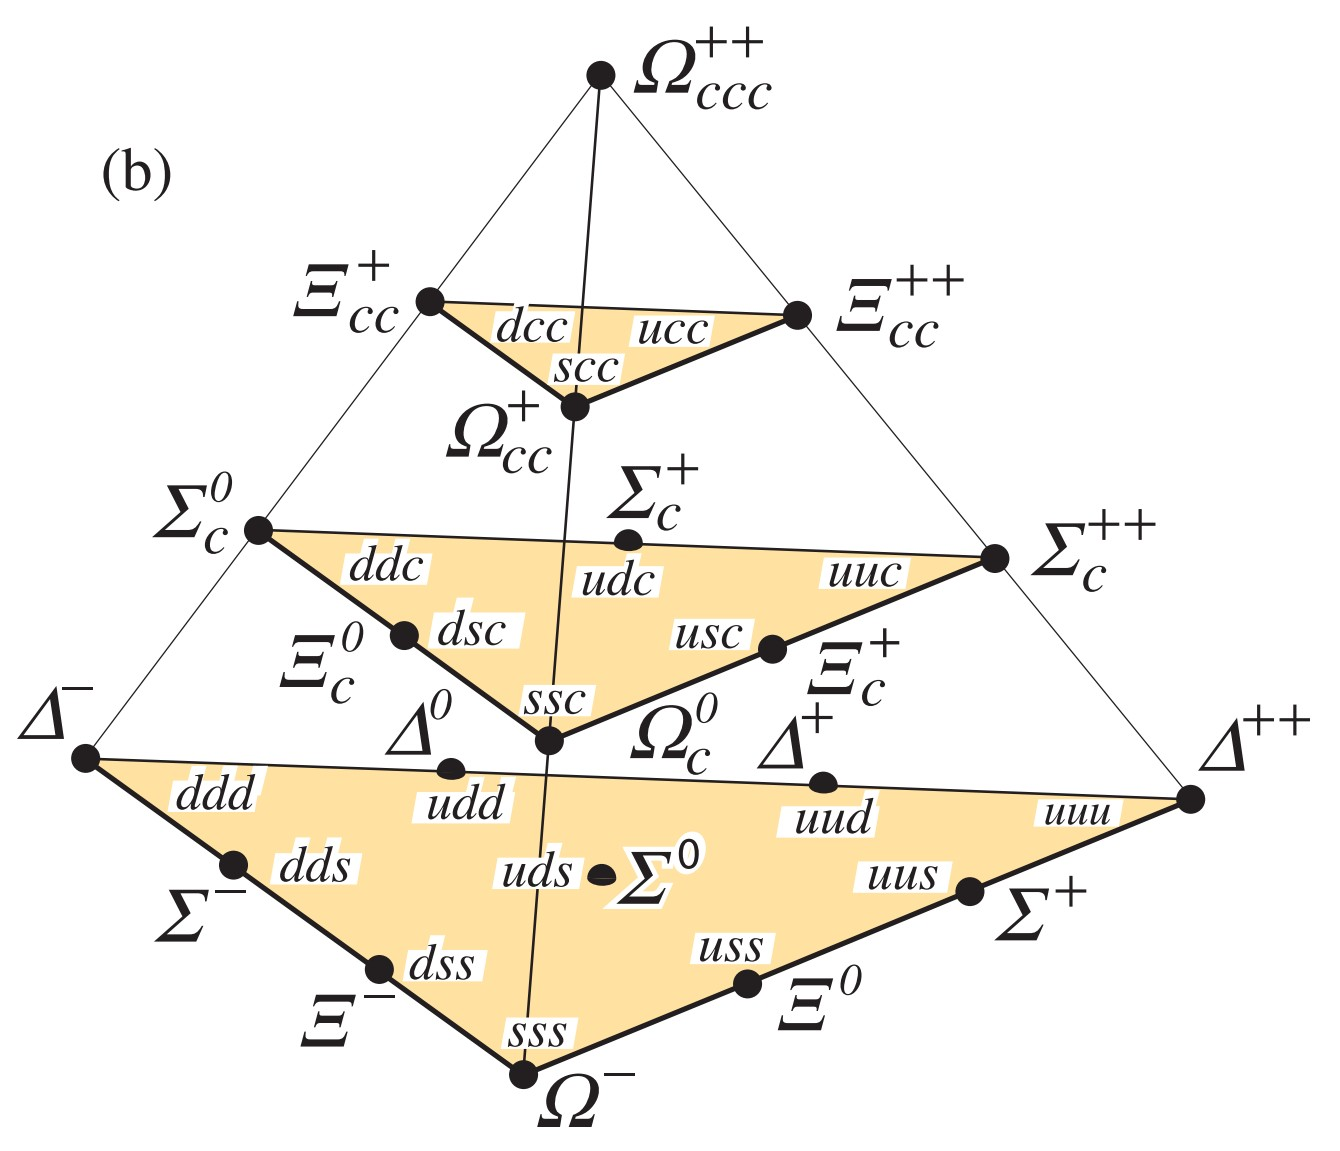
\includegraphics[width=\linewidth, height=0.7\textheight, keepaspectratio]{Images/594e59cc-d7ab-4a37-ad49-f782ae1831bc.jpg}
        \caption{Das 20-Plet mit einem SU$_3$ Dekuplett.\\\scriptsize\parencite{C.Amsler.2017}}
        \end{figure}
      \end{minipage}
      \hfill
      \begin{minipage}{0.38\textwidth}
        \begin{itemize}
          \item Erweiterung des SU$_3$ Dekupletts
          \item weitere Dimension: Charm
          \item Neue, schwere Hadronen
            \end{itemize}
          \end{minipage}
      \end{frame}

              \begin{frame}{Gell-Mann: Zusammensetzung der Hadronen}
                \begin{figure}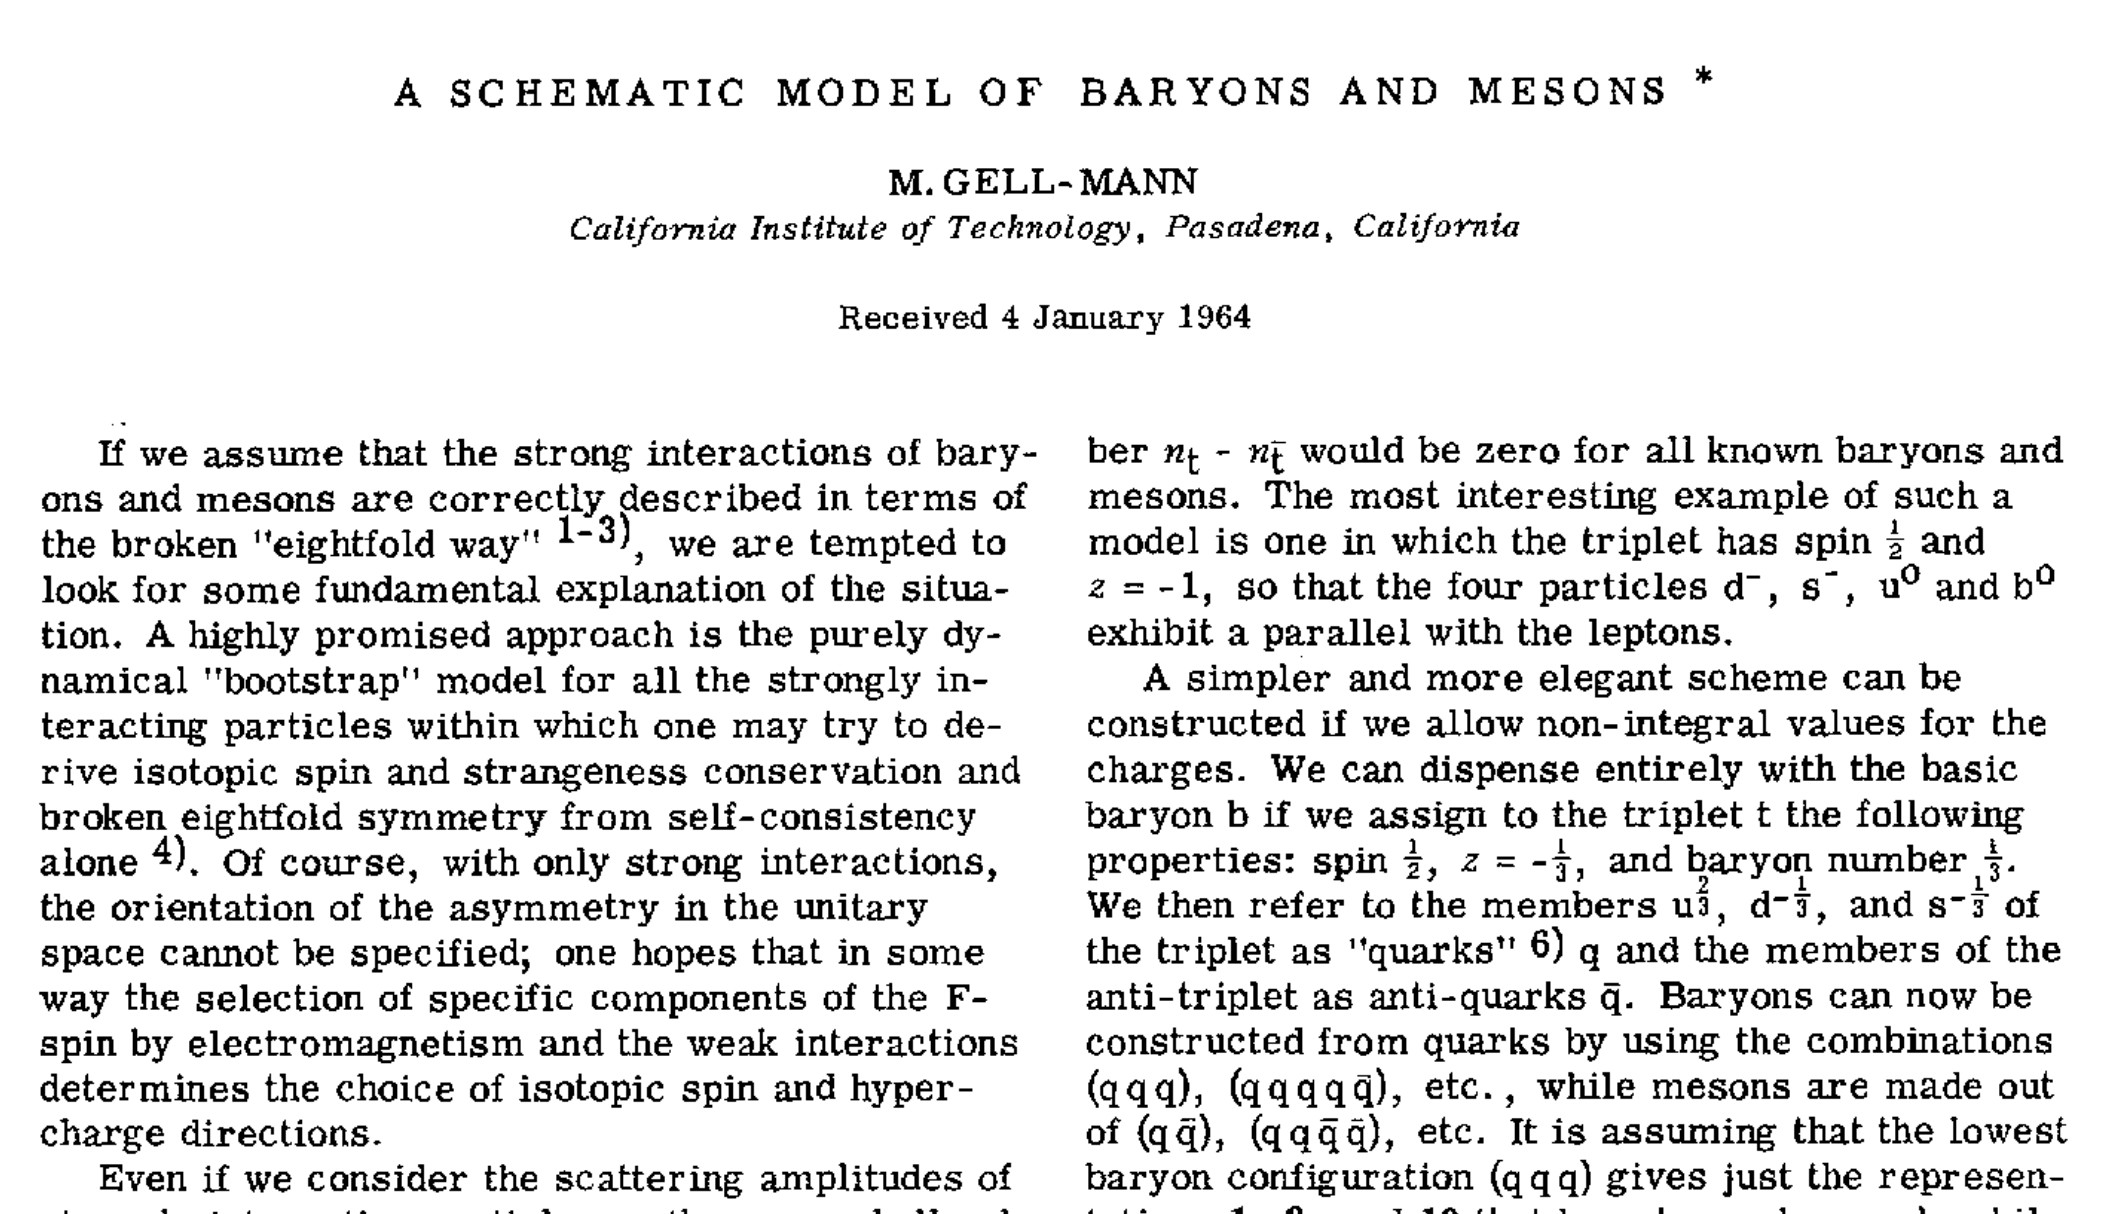
\includegraphics[height=0.85\textheight, width=\textwidth, keepaspectratio]{Images/8ad56d13-e301-4a37-be9c-7077ac16ce16.jpg}\\\small\cite[S.~214]{GellMann.1964}\end{figure}
                \begin{tikzpicture}[remember picture, overlay]
            \fill[yellow, opacity=0.3] (7, 1.9) rectangle (12.8, 2.7);
                \end{tikzpicture}
    \end{frame}

    \section{Die Suche nach Pentaquarks}

    \begin{frame}{Pentaquarks: Theoretische Vorhersagen}
      \begin{itemize}
        \item Gell-Manns Idee von \citeyear{GellMann.1964} durch \textcite{Hogaasen.1978,Strottman.1979} erweitert:
        \begin{itemize}
          \item Pentaquarks: $qqqq\bar{q}$
          \item Lipkin erfand den Begriff Pentaquark \parencite{Lipkin.1987}
        \end{itemize}
        \item LHCb: Untersuchung von Λ\textsubscript{b}\textsuperscript{0}→J/ψK\textsuperscript{-}p Zerfällen durch \textcite{Aaij.2015}.
        \item Zerfälle könnten minimalen Quarkanteil von $c\bar{c}uud$ enthalten. \\ $\rightarrow$ Charmonium Pentaquarks ($P_c^+$)
      \end{itemize}
    \end{frame}

    \begin{frame}{Zerfallskanäle von Λ\textsubscript{b}\textsuperscript{0}→J/ψ  K\textsuperscript{-}  p}
      \begin{figure}[htb]
          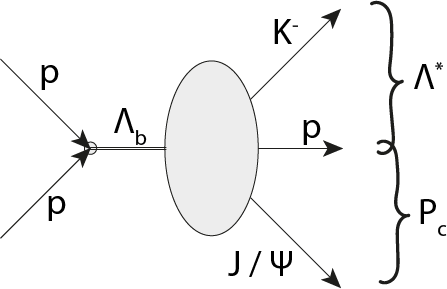
\includegraphics[width=0.22\textwidth]{FeynmanDiag/Gesamt.png}\\[1em]
          \centering
          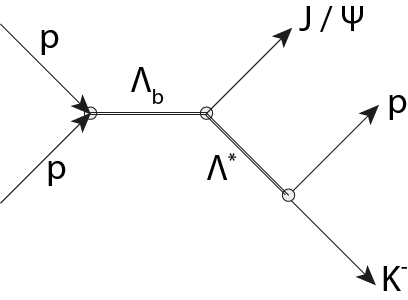
\includegraphics[width=0.3\textwidth]{FeynmanDiag/Lambda.png}
          \hspace{3cm}
          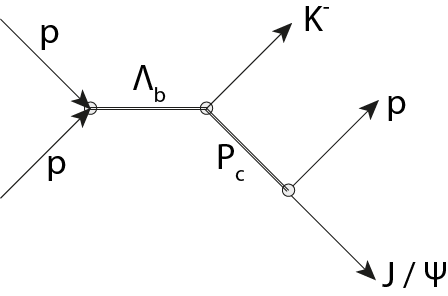
\includegraphics[width=0.3\textwidth]{FeynmanDiag/pentaquark.png}
          \caption{Feynmandiagramme der Zerfallskanäle von Λ\textsubscript{b}\textsuperscript{0} in J/ψ  K\textsuperscript{-}  p\\\scriptsize \emph{Eigene Darstellung nach Daten von \textcite{Aaij.2015}}}
      \end{figure}
  \end{frame}



    \begin{frame}{\textcolor{red}{resultat der LHCb 2015 Messungen}}
      \begin{figure}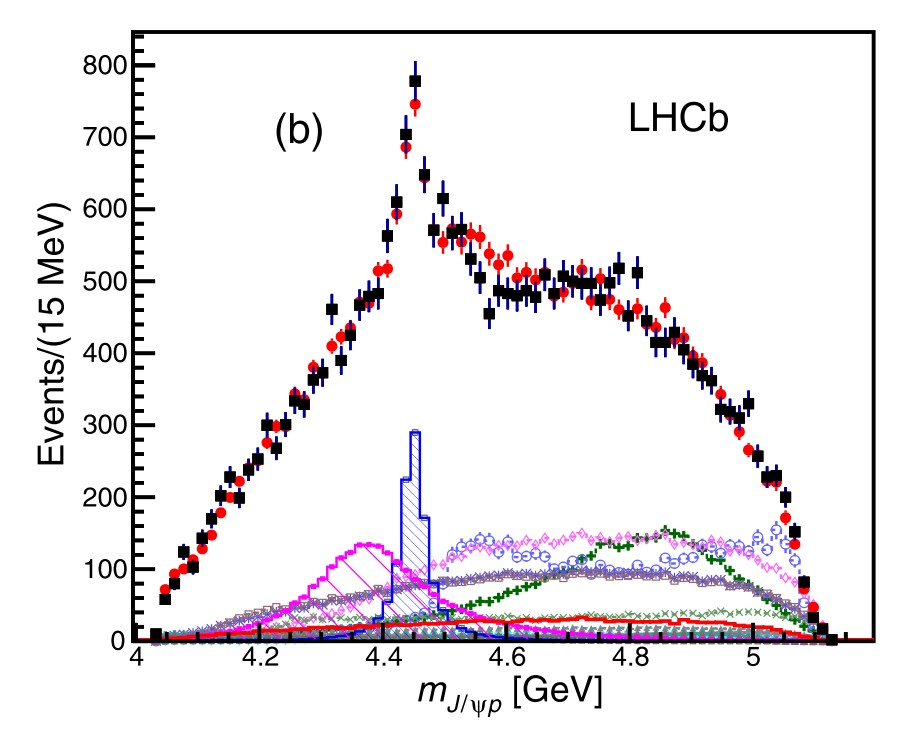
\includegraphics[width=\textwidth, height=0.6\textheight, keepaspectratio]{Images/f4773e9d-39b6-4dc8-8301-4f91e5c718c3.jpg}%\caption{Aaij, Adeva et al 2015 - Observation of J ψp Resonances Consistent.jpg}
        \\\protect\cite[S.~2]{Aaij.2015}\end{figure}
      \begin{itemize}
        \item \emph{\textcolor{red}{leider noch nicht so genau?}}
      \end{itemize}
    \end{frame}

    \begin{frame}{Pentaquarks: Weitere Entdeckungen}
      \begin{itemize}
        \item LHCb: Entdeckung von $P_c^+(4312)$ und $P_c^+(4450)$ durch \textcite{Aaij.2019}
        \item Zerfälle von $P_c^+$ in $J/\psi p$ und $J/\psi p\pi$-Kanälen
        \item Hinweise auf weitere Pentaquarks
      \end{itemize}
      \emph{\textcolor{red}{\textbf{A narrow pentaquark state is discovered with a statistical significance of $7.3\sigma$
            }}}
    \end{frame}


      \begin{frame}{\textcolor{red}{Ergebnisse der LHCb 2019 Messungen - ?? weiter}}
        \begin{minipage}{0.48\textwidth}
          \begin{figure}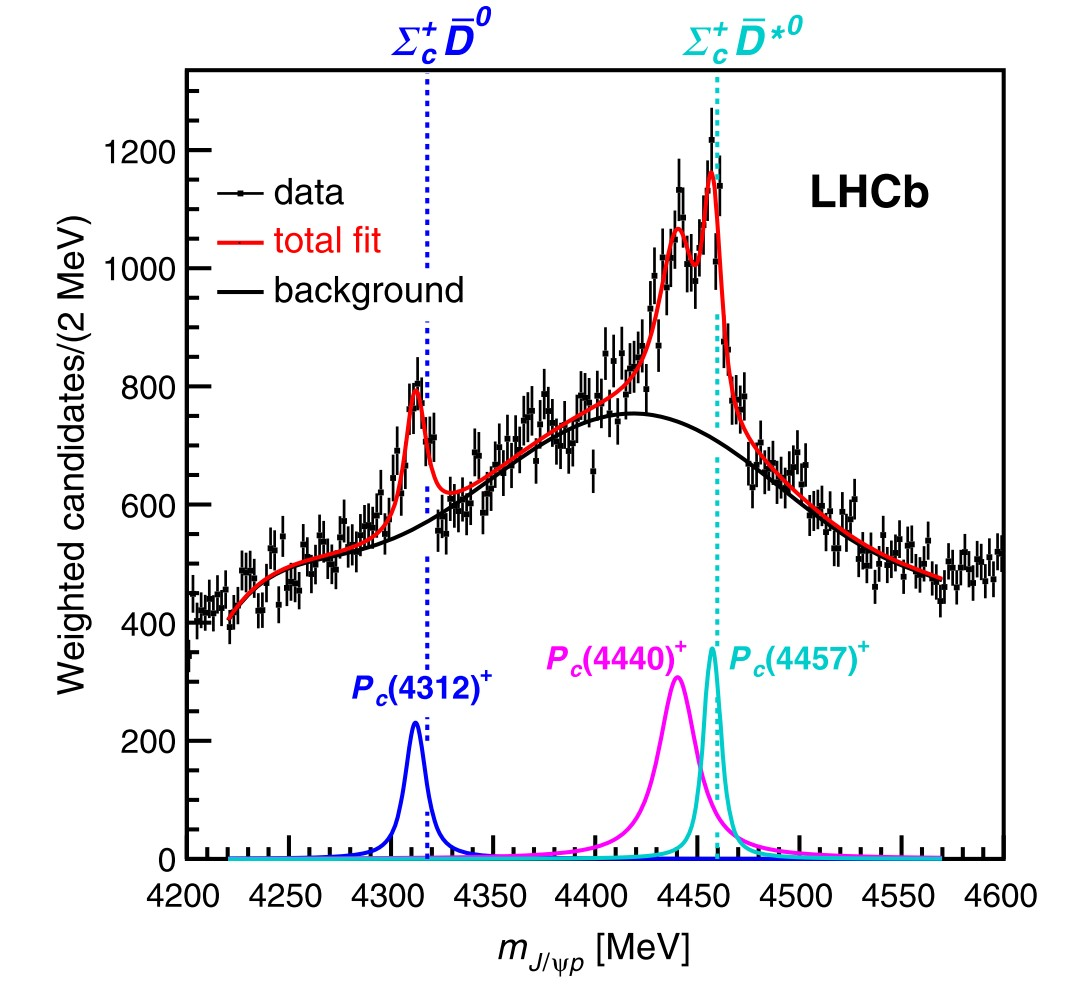
\includegraphics[width=\textwidth]{Images/76e29612-a8a4-4650-8573-5e331d33a362.jpg}%\caption{Aaij, Abellán Beteta et al 2019 - Observation of a Narrow Pentaquark - total fit}
            \\\protect\cite[S.~4]{Aaij.2019}\end{figure}
        \end{minipage}
        \hfill
        \begin{minipage}{0.48\textwidth}
          \begin{figure}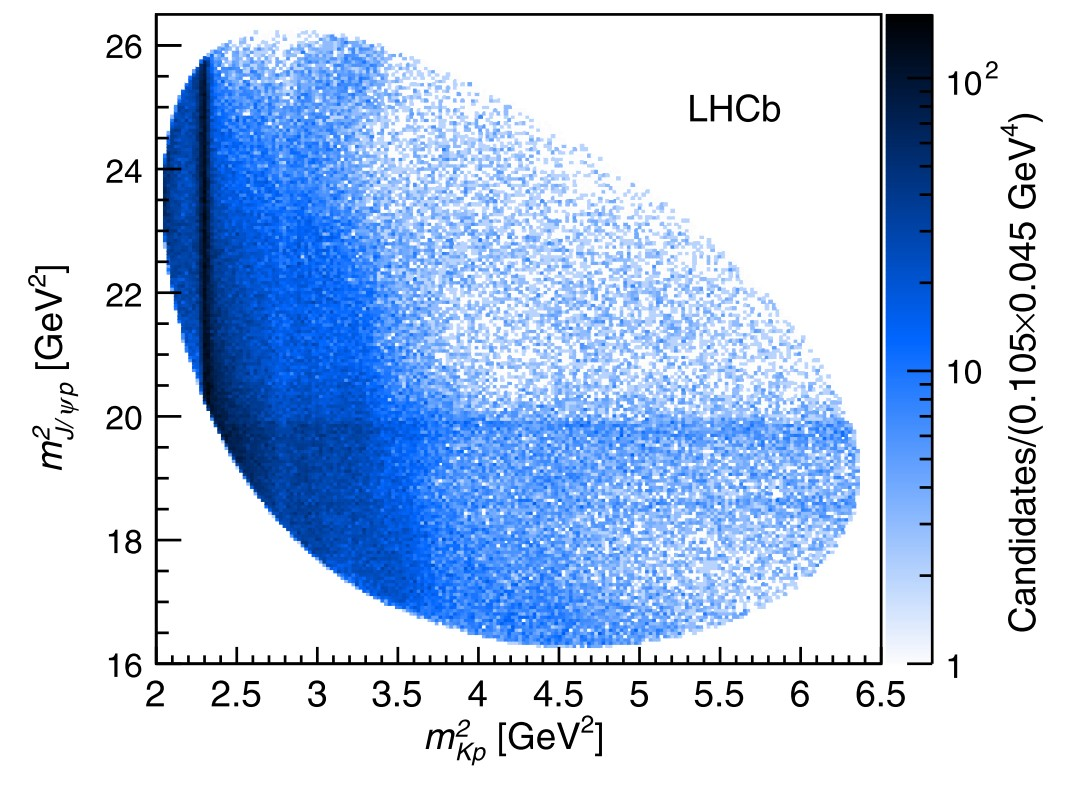
\includegraphics[width=\textwidth]{Images/e4479e29-be8d-4b9c-bfc4-f1747ace3818.jpg}%\caption{Aaij, Abellán Beteta et al 2019 - Daalitz}
            \\\protect\cite[S.~2]{Aaij.2019}\end{figure}
        \end{minipage}
      \end{frame}
    
    \section{Schluss \& Ausblick}
    \begin{frame}{Schluss \& Ausblick}
      \begin{itemize}
        \item \textcolor{red}{Zusammenfassung der wichtigsten Punkte}
        \item Ausblick auf weitere Forschungsrichtungen?
      \end{itemize}
    \end{frame}

    % Thank You Slide
    \begin{frame}
      \begin{center}
          \Huge Vielen Dank!
      \end{center}
  \end{frame}

    % Bibliography    
    \begin{frame}[allowframebreaks, noframenumbering, plain]{Literaturverzeichnis}
   \printbibliography%[nottype=unpublished]
    \end{frame}

    % Black slide
    \begin{frame}[plain, noframenumbering]
        \begin{tikzpicture}[remember picture, overlay]
            \fill[black] (current page.south west) rectangle (current page.north east);
        \end{tikzpicture}
        Test~\cite{Aaij.2015,Aaij.2019,C.Amsler.2017,GellMann.1964,Zweig.1964,Zweig.1964b}
    \end{frame}

\end{document}
